
%(BEGIN_QUESTION)
% Copyright 2011, Tony R. Kuphaldt, released under the Creative Commons Attribution License (v 1.0)
% This means you may do almost anything with this work of mine, so long as you give me proper credit

A data acquisition system consisting of three DAQ modules connected to a personal computer using RS-485 (multidrop) through a modem has a problem.  The DAQ software running in the personal computer does not seem to ``recognize'' DAQ \#1, although it does recognize the other two DAQ modules and is receiving data from them:

$$\includegraphics[width=15.5cm]{i00888x01.eps}$$

Looking at the LED indicators, you notice that the green ``Rx'' LEDs on all three DAQ units blink.  You also notice that the red ``Tx'' LEDs on DAQ modules \#2 and \#3 are blinking as well, but that the ``Tx'' LED on DAQ \#1 is constantly off.

Identify the likelihood of each specified fault for this system.  Consider each fault one at a time (i.e. no coincidental faults), determining whether or not each fault could independently account for {\it all} measurements and symptoms in this network.

% No blank lines allowed between lines of an \halign structure!
% I use comments (%) instead, so that TeX doesn't choke.

$$\vbox{\offinterlineskip
\halign{\strut
\vrule \quad\hfil # \ \hfil & 
\vrule \quad\hfil # \ \hfil & 
\vrule \quad\hfil # \ \hfil \vrule \cr
\noalign{\hrule}
%
% First row
{\bf Fault} & {\bf Possible} & {\bf Impossible} \cr
%
\noalign{\hrule}
%
% Another row
Open cable between DAQ \#1 and DAQ \#2 &  &  \cr
%
\noalign{\hrule}
%
% Another row
Open cable between DAQ \#2 and DAQ \#3 &  &  \cr
%
\noalign{\hrule}
%
% Another row
Open cable between DAQ \#3 and modem &  &  \cr
%
\noalign{\hrule}
%
% Another row
Incorrect serial settings (e.g. parity, bit rate) in DAQ \#1 &  &  \cr
%
\noalign{\hrule}
%
% Another row
Incorrect serial settings (e.g. parity, bit rate) in DAQ \#2 &  &  \cr
%
\noalign{\hrule}
%
% Another row
Incorrect serial settings (e.g. parity, bit rate) in DAQ \#3 &  &  \cr
%
\noalign{\hrule}
%
% Another row
Incorrect serial settings (e.g. parity, bit rate) in computer &  &  \cr
%
\noalign{\hrule}
%
% Another row
Missing termination resistor &  &  \cr
%
\noalign{\hrule}
} % End of \halign 
}$$ % End of \vbox



\vskip 20pt \vbox{\hrule \hbox{\strut \vrule{} {\bf Suggestions for Socratic discussion} \vrule} \hrule}

\begin{itemize}
\item{} Identify how a digital multimeter (DMM) could be used to perform useful diagnostic tests in an RS-485 network such as this.  What sorts of things can we measure using a DMM connected to a digital network?  What sorts of things {\it can't} we measure using a DMM connected to a digital network?
\end{itemize}

\underbar{file i00888}
%(END_QUESTION)





%(BEGIN_ANSWER)


%(END_ANSWER)





%(BEGIN_NOTES)

DAQ \#1 is receiving data, but never transmitting.  Either it has a transmitter problem, or else it cannot understand the data it's receiving and thus never replies.

% No blank lines allowed between lines of an \halign structure!
% I use comments (%) instead, so that TeX doesn't choke.

$$\vbox{\offinterlineskip
\halign{\strut
\vrule \quad\hfil # \ \hfil & 
\vrule \quad\hfil # \ \hfil & 
\vrule \quad\hfil # \ \hfil \vrule \cr
\noalign{\hrule}
%
% First row
{\bf Fault} & {\bf Possible} & {\bf Impossible} \cr
%
\noalign{\hrule}
%
% Another row
Open cable between DAQ \#1 and DAQ \#2 &  & $\surd$ \cr
%
\noalign{\hrule}
%
% Another row
Open cable between DAQ \#2 and DAQ \#3 &  & $\surd$ \cr
%
\noalign{\hrule}
%
% Another row
Open cable between DAQ \#3 and modem &  & $\surd$ \cr
%
\noalign{\hrule}
%
% Another row
Incorrect serial settings (e.g. parity, bit rate) in DAQ \#1 & $\surd$ &  \cr
%
\noalign{\hrule}
%
% Another row
Incorrect serial settings (e.g. parity, bit rate) in DAQ \#2 &  & $\surd$ \cr
%
\noalign{\hrule}
%
% Another row
Incorrect serial settings (e.g. parity, bit rate) in DAQ \#3 &  & $\surd$ \cr
%
\noalign{\hrule}
%
% Another row
Incorrect serial settings (e.g. parity, bit rate) in computer &  & $\surd$ \cr
%
\noalign{\hrule}
%
% Another row
Missing termination resistor &  & $\surd$ \cr
%
\noalign{\hrule}
} % End of \halign 
}$$ % End of \vbox


%INDEX% Troubleshooting review: electric circuits

%(END_NOTES)


